% *********************************************************************
% © 2010–2026 Jeremy Sylvestre
%
% Permission is granted to copy, distribute and/or modify this document
% under the terms of the GNU Free Documentation License, Version 1.3 or
% any later version published by the Free Software Foundation; with no
% Invariant Sections, no Front-Cover Texts, and no Back-Cover Texts. A
% copy of the license is included in the appendix entitled “GNU Free
% Documentation License” that appears in the output document of this
% PreTeXt source code. All trademarks™ are the registered® marks of
% their respective owners.
%
% *********************************************************************

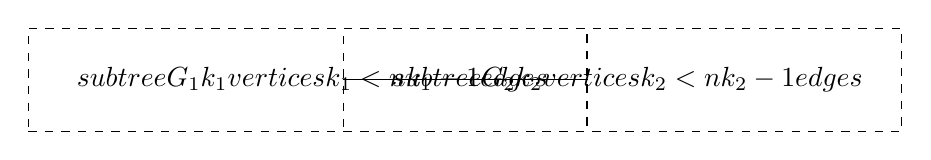
\begin{tikzpicture}[
	vertex/.style={ circle, draw, very thin, fill, inner sep=0pt, minimum size=4pt },
	vertexg/.style={ black!40!white, circle, draw, very thin, fill, inner sep=0pt, minimum size=4pt },
	vertexo/.style={ circle, draw, very thin, inner sep=0pt, minimum size=4pt }
]

\node at (-2,0) (g1) [rectangle=gray,draw,dashed,inner sep=0.5cm] {$
	\begin{matrix}
		\text{subtree } G_1 \\
		k_1 \text{ vertices}\\
		k_1 < n \lgcimplies \\
		k_1 - 1 \text{ edges}
	\end{matrix}
$};
\node at (2,0) (g2) [rectangle=gray,draw,dashed,inner sep=0.5cm] {$
	\begin{matrix}
		\text{subtree } G_2 \\
		k_2 \text{ vertices}\\
		k_2 < n \lgcimplies \\
		k_2 - 1 \text{ edges}
	\end{matrix}
$};
\draw (g1.east) to (g2.west);

\end{tikzpicture}
